\documentclass[11pt,a4paper]{article}

\usepackage{fontspec}
% Using default LaTeX font (Latin Modern / Computer Modern)

\usepackage[margin=1.8cm]{geometry}
\usepackage{xcolor}
\usepackage{graphicx}
\usepackage{amsmath,amsfonts,amssymb}
\usepackage{booktabs}
\usepackage{tabularx}
\usepackage{longtable}
\usepackage{array}
\usepackage{fancyhdr}
\usepackage{tcolorbox}
\usepackage{listings}
\usepackage[hidelinks,colorlinks=true,linkcolor=blue!70!black,urlcolor=blue!70!black,citecolor=blue!70!black]{hyperref}

% Define color palette
\definecolor{primary}{RGB}{18, 52, 86}
\definecolor{secondary}{RGB}{30, 144, 255}
\definecolor{darkred}{RGB}{180, 20, 20}
\definecolor{darkgreen}{RGB}{20, 130, 20}
\definecolor{lightgray}{RGB}{247, 249, 251}
\definecolor{bordergray}{RGB}{210, 215, 225}

% Header & Footer
\pagestyle{fancy}
\fancyhf{}
\fancyhead[L]{\small\textbf{HW02 – Domain Testing on EShop}}
\fancyhead[R]{\small\textsl{Khoa CNTT – ĐH Khoa Học Tự Nhiên, ĐHQG-HCM}}
\fancyfoot[C]{\thepage}
\renewcommand{\headrulewidth}{0.5pt}

% Define JavaScript for listings
\lstdefinelanguage{JavaScript}{
  keywords={typeof, new, true, false, catch, function, return, null, switch, var, if, in, while, do, else, case, break, const, let, async, await},
  keywordstyle=\color{blue}\bfseries,
  ndkeywords={class, export, boolean, throw, implements, import, this},
  ndkeywordstyle=\color{primary}\bfseries,
  identifierstyle=\color{black},
  sensitive=false,
  comment=[l]{//},
  morecomment=[s]{/*}{*/},
  commentstyle=\color{gray}\itshape,
  stringstyle=\color{darkgreen},
  morestring=[b]',
  morestring=[b]"
}

\lstset{
    language=JavaScript,
    basicstyle=\ttfamily\footnotesize,
    backgroundcolor=\color{lightgray},
    frame=single,
    rulecolor=\color{bordergray},
    breaklines=true,
    breakatwhitespace=true,
    tabsize=2,
    showstringspaces=false
}

\tcbuselibrary{skins,breakable}
\newtcolorbox{infobox}[1][]{
    colback=lightgray,
    colframe=primary,
    fonttitle=\bfseries\color{white},
    coltitle=white,
    title=#1,
    arc=2mm,
    boxrule=1pt,
    breakable
}

\newcolumntype{L}[1]{>{\raggedright\arraybackslash}p{#1}}
\newcolumntype{Y}{>{\raggedright\arraybackslash}X}

\begin{document}

% ==================== TITLE PAGE ====================
\begin{titlepage}
    \centering
    \vspace*{1.5cm}
    {\large \textbf{ĐẠI HỌC KHOA HỌC TỰ NHIÊN -- ĐHQG-HCM}}\\[0.2cm]
    {\large \textbf{KHOA CÔNG NGHỆ THÔNG TIN}}\\[0.4cm]
    \rule{0.6\textwidth}{0.8pt}\\[2.5cm]

    {\Large \textbf{BÁO CÁO BÀI TẬP VỀ NHÀ (HW02)}}\\[0.5cm]
    {\LARGE \textbf{KIỂM THỬ MIỀN VÀ PHÂN TÍCH GIÁ TRỊ BIÊN}}\\[0.3cm]
    {\Large \textbf{HỆ THỐNG THƯƠNG MẠI ĐIỆN TỬ ESHOP (SUT)}}\\[0.3cm]
    {\normalsize \textsl{Domain Testing \& Boundary Value Analysis}}\\[2.5cm]

    \begin{minipage}{0.75\textwidth}
        \normalsize
        \renewcommand{\arraystretch}{1.3}
        \begin{tabular}{ll}
            \textbf{Môn học:} & Kiểm thử phần mềm nâng cao (CS423) \\
            \textbf{Sinh viên thực hiện:} & Nguyễn Bảo An \\
            \textbf{Mã số sinh viên (MSSV):} & 23120207 \\
            \textbf{Kho mã nguồn GitHub:} & \url{https://github.com/NgBaoAnn/hw02-domain-testing} \\
            \textbf{Trang GitHub Issues:} & \url{https://github.com/NgBaoAnn/hw02-domain-testing/issues} \\
            \textbf{Giảng viên hướng dẫn:} & TS. Lâm Quang Vũ \\
            & TS. Trần Duy Hoàng \\
            & ThS. Trần Thị Bích Hạnh \\
            & ThS. Trương Phước Lộc \\
            & ThS. Hồ Tuấn Thanh \\
            \textbf{Ngày nộp báo cáo:} & 15/10/2026 \\
        \end{tabular}
    \end{minipage}

    \vfill
    {\normalsize TP. HỒ CHÍ MINH, THÁNG 10/2026}
    \vspace*{1cm}
\end{titlepage}

% ==================== TABLE OF CONTENTS ====================
\tableofcontents
\newpage

% ==================== SECTION 1 ====================
\section{Giới Thiệu Tổng Quan \& Phạm Vi Phân Công}

Hệ thống Thương mại Điện tử \textbf{EShop} là một ứng dụng web/mobile full-stack phục vụ thực hành kiểm thử phần mềm chất lượng cao, bao gồm:
\begin{itemize}
    \item \textbf{Backend REST API:} Node.js, Express framework, SQLite3 database (\texttt{backend/server.js}, cổng 3000).
    \item \textbf{Web Frontend:} React 18, Vite, React Router, TailwindCSS (\texttt{frontend-web/}, cổng 5173).
    \item \textbf{Web Admin Portal:} React 18, Vite, TailwindCSS (\texttt{frontend-admin/}, cổng 5174).
    \item \textbf{Mobile Client:} React Native / Expo (\texttt{frontend-mobile/App.js}).
\end{itemize}

Theo quy định tại Mục 5 của đề bài (mỗi sinh viên chọn 4 tính năng độc lập từ 4 nhóm nghiệp vụ khác nhau, bảo đảm không trùng lặp trong nhóm), bài tập này tập trung thiết kế và thực thi kiểm thử toàn diện trên 4 tính năng sau:

\begin{table}[h]
\centering
\small
\begin{tabularx}{\textwidth}{L{3.2cm} L{2.2cm} L{4.5cm} Y}
\toprule
\textbf{Nhóm (Pool)} & \textbf{Mã tính năng} & \textbf{Tên tính năng} & \textbf{Phạm vi mã nguồn SUT} \\
\midrule
\textbf{Pool A (Auth \& SP)} & \textbf{FR-06} & Chi tiết sản phẩm \& Thêm vào giỏ & \texttt{ProductDetail.jsx}, \texttt{server.js} (\texttt{/api/products/:id}) \\
\textbf{Pool B (Giỏ \& Đơn)} & \textbf{FR-11} & Lịch sử đơn hàng của người dùng & \texttt{Profile.jsx}, \texttt{server.js} (\texttt{/api/orders}) \\
\textbf{Pool C (Web Admin)} & \textbf{FR-19} & Quản lý người dùng dành cho Admin & \texttt{frontend-admin/App.jsx}, \texttt{server.js} (\texttt{/api/admin/users}) \\
\textbf{Pool D (Mobile App)} & \textbf{Mobile FR-10} & Hủy đơn hàng trên ứng dụng di động & \texttt{frontend-mobile/App.js} (\texttt{cancelOrder}) \\
\bottomrule
\end{tabularx}
\caption{Bảng 4 tính năng được lựa chọn kiểm thử}
\end{table}

Mục tiêu cốt lõi của đợt kiểm thử này là áp dụng nghiêm ngặt các nguyên lý \textbf{Kiểm thử Miền (Domain Testing)} và \textbf{Phân tích Giá trị Biên (Boundary Value Analysis)} theo chuẩn công nghiệp ISTQB, kết hợp khai thác sức mạnh của AI Agent một cách có kỷ luật (Human-in-the-Loop) để rà quét triệt để các góc khuất, logic bẫy mã nguồn (seeded bugs), lỗi phân quyền (Broken Object Level Authorization - BOLA), và các bất cập về trải nghiệm người dùng (UX).

% ==================== SECTION 2 ====================
\section{Phương Pháp Luận Kiểm Thử (Testing Methodology)}

\subsection{Phân vùng tương đương (Equivalence Partitioning - EP)}
Kỹ thuật phân vùng tương đương chia toàn bộ miền giá trị đầu vào của một trường hoặc tham số thành các tập con rời rạc (partitions), với giả định rằng mọi giá trị trong cùng một phân vùng sẽ được hệ thống xử lý hoàn toàn như nhau:
\begin{itemize}
    \item \textbf{Phân vùng Hợp lệ (Valid Equivalence Partition - VEP):} Tập hợp các giá trị được hệ thống chấp nhận theo đúng đặc tả nghiệp vụ SRS.
    \item \textbf{Phân vùng Không hợp lệ (Invalid Equivalence Partition - IEP):} Tập hợp các giá trị vi phạm ràng buộc về kiểu dữ liệu, định dạng, độ dài, hoặc giới hạn logic mà hệ thống bắt buộc phải từ chối hoặc trả về thông báo lỗi thích hợp.
\end{itemize}

\subsection{Phân tích giá trị biên (Boundary Value Analysis - BVA)}
Kinh nghiệm kiểm thử phần mềm thực tế chứng minh phần lớn lỗi tiềm ẩn tập trung tại các đường biên ngăn cách giữa các phân vùng tương đương. Chúng tôi triển khai kết hợp cả hai kỹ thuật biên chuẩn:
\begin{enumerate}
    \item \textbf{2-point BVA:} Với mỗi biên, khảo sát 2 điểm:
    \begin{itemize}
        \item \textbf{On-point:} Giá trị nằm chính xác ngay trên đường ranh giới.
        \item \textbf{Off-point:} Giá trị nằm ngay sát cạnh đường ranh giới nhưng thuộc về phía đối diện (ngoài vùng hợp lệ).
    \end{itemize}
    \item \textbf{3-point BVA (Extended Boundary Testing):} Khảo sát 3 điểm gồm $\{\text{Biên} - 1, \text{Biên}, \text{Biên} + 1\}$ (hoặc On, In, Out) nhằm bảo đảm không xảy ra lỗi lệch 1 (Off-by-one errors: $<$ thay vì $\le$, $>$ thay vì $\ge$).
    \item \textbf{Phân tích biên chuyển trạng thái (State Transition Boundaries):} Khảo sát các điểm trạng thái hợp lệ và bất hợp lệ khi kích hoạt hành động nghiệp vụ (ví dụ: chuyển đổi trạng thái đơn hàng).
\end{enumerate}

\subsection{Chiến lược ưu tiên AI có kiểm soát (AI-First \& Human-in-the-Loop)}
Tuân thủ nghiêm ngặt nguyên tắc chỉ đạo:
\begin{itemize}
    \item Sử dụng AI để tăng tốc phân tích cấu trúc mã nguồn và sinh kịch bản ban đầu.
    \item Kiểm thử viên con người trực tiếp rà soát, viết test script tự động (\texttt{tests/}), chạy thực thi trên SUT và chụp ảnh bằng chứng lỗi thực tế.
    \item Thực hiện phân tích khoảng trống AI (AI Gap Analysis) để phát hiện các điểm AI thiên kiến hoặc bỏ sót.
\end{itemize}

\newpage

% ==================== SECTION 3 ====================
\section{Tính Năng A (FR-06): Xem Chi Tiết Sản Phẩm \& Thêm Vào Giỏ}

\subsection{Phân tích miền biến \& Không gian trạng thái}
\begin{itemize}
    \item \textbf{Biến $Q$ (\texttt{quantity}):}
    \begin{itemize}
        \item Miền hợp lệ: $Q \in \mathbb{Z}^+, 1 \le Q \le \text{MaxQty}$.
        \item Miền không hợp lệ: $Q \le 0$ (số âm, số 0), số thực không nguyên ($1.5$), giá trị phi số (\texttt{abc}, \texttt{null}, \texttt{NaN}).
        \item Giá trị biên khảo sát:
        \begin{itemize}
            \item Biên dưới: $0$ (Off-point, Invalid), $1$ (On-point, Valid), $2$ (In-point, Valid).
            \item Biên âm: $-1$ (Negative Boundary).
        \end{itemize}
    \end{itemize}
    \item \textbf{Biến $C$ (\texttt{clickCount}):} Trạng thái số lần bấm nút. Mong đợi $C=1$ là thêm vào giỏ.
\end{itemize}

\subsection{Ma trận kiểm thử miền \& Phân tích giá trị biên (FR-06)}

\begin{table}[h]
\centering
\footnotesize
\begin{tabularx}{\textwidth}{l L{2.2cm} L{1.8cm} L{3cm} Y c}
\toprule
\textbf{Mã TC} & \textbf{Kỹ thuật} & \textbf{Đầu vào} & \textbf{Kỳ vọng (SRS)} & \textbf{Thực tế trên SUT (Actual)} & \textbf{Kết luận} \\
\midrule
TC-FR06-01 & BVA On-point & $Q = 1$ & Thêm 1 SP vào giỏ & Thêm thành công (cần 2 click) & \textbf{PASS*} \\
TC-FR06-02 & BVA In-point & $Q = 2$ & Thêm 2 SP vào giỏ & Thêm 2 SP vào giỏ & \textbf{PASS} \\
TC-FR06-03 & BVA Off-point & $Q = 0$ & Báo lỗi, yêu cầu $Q \ge 1$ & \textbf{SUT thêm $Q=0$ vào giỏ!} & \textbf{\color{darkred}FAIL (BUG-02)} \\
TC-FR06-04 & Domain Số âm & $Q = -1$ & Báo lỗi số lượng âm & \textbf{SUT nhận $Q=-1$, trừ tiền giỏ!} & \textbf{\color{darkred}FAIL (BUG-02)} \\
TC-FR06-05 & Domain Ký tự & $Q = \text{"abc"}$ & Chặn nhập ký tự & Lưu $Q=\text{NaN}$ vào giỏ hàng & \textbf{\color{darkred}FAIL (BUG-02)} \\
TC-FR06-06 & UX Bấm lần 1 & Click 1 & Thêm vào giỏ ngay & \textbf{Bị nuốt sự kiện, không phản hồi} & \textbf{\color{darkred}FAIL (BUG-01)} \\
TC-FR06-07 & UX Bấm lần 2 & Click 2 & Thêm vào giỏ & Thêm vào giỏ, đổi chữ nút & \textbf{PASS} \\
TC-FR06-08 & API ID lẻ & ID $= 1$ & Price dạng \texttt{number} & Price dạng \texttt{number} & \textbf{PASS} \\
TC-FR06-09 & API ID chẵn & ID $= 2$ & Price dạng \texttt{number} & \textbf{Price dạng string ("28000000")} & \textbf{\color{darkred}FAIL (Backend)} \\
TC-FR06-10 & API Không tồn tại & ID $= 9999$ & HTTP 404 Not Found & HTTP 200 kèm \texttt{\{\}} & \textbf{\color{darkred}FAIL (REST Bug)} \\
\bottomrule
\end{tabularx}
\caption{Ma trận kiểm thử FR-06 trên hệ thống SUT}
\end{table}

\subsection{Kết quả thực thi kiểm thử \& Xác nhận lỗi thực tế}
Kịch bản tự động \texttt{node tests/verify\_fr06.js} xác nhận 100\% các lỗi:
\begin{lstlisting}[caption={Đoạn mã bẫy sự kiện click tại ProductDetail.jsx:21-25}]
const handleAddToCart = () => {
  if (clickCount === 0) {
    setClickCount(1);
    return; // BẪY: Lần bấm đầu tiên bị nuốt hoàn toàn, không gọi addToCart()!
  }
  addToCart(product, parseInt(quantity));
  setAdded(true);
};
\end{lstlisting}

\subsection{Phân tích khoảng trống AI (AI Gap Analysis - FR-06)}
AI thường mắc lỗi \textit{Happy-Path Bias}: giả định rằng hàm \texttt{handleAddToCart} luôn gọi trực tiếp \texttt{addToCart}. AI không nhận ra bẫy \texttt{clickCount === 0} nếu con người không chỉ định đọc từng dòng lệnh logic stateful.

\newpage

% ==================== SECTION 4 ====================
\section{Tính Năng B (FR-11): Lịch Sử Đơn Hàng \& Hủy Đơn Hàng}

\subsection{Phân tích máy trạng thái đơn hàng (Order State Machine)}
Vòng đời trạng thái đơn hàng theo đặc tả SRS:
$$\text{pending} \xrightarrow{\text{admin}} \text{confirmed} \xrightarrow{\text{admin}} \text{shipping} \xrightarrow{\text{admin}} \text{delivered}$$
$$\text{pending / confirmed} \xrightarrow{\text{user cancel}} \text{canceled}$$
\textbf{Ràng buộc SRS:} Người dùng chỉ được phép hủy đơn khi trạng thái là \texttt{pending} hoặc \texttt{confirmed}. Khi đơn đã chuyển sang \texttt{shipping} hoặc \texttt{delivered}, hành động hủy đơn bắt buộc phải bị từ chối với HTTP 400.

\subsection{Ma trận kiểm thử miền \& BVA (FR-11)}

\begin{table}[h]
\centering
\footnotesize
\begin{tabularx}{\textwidth}{l L{2.2cm} L{1.8cm} L{3cm} Y c}
\toprule
\textbf{Mã TC} & \textbf{Kỹ thuật} & \textbf{Trạng thái} & \textbf{Kỳ vọng (SRS)} & \textbf{Thực tế trên SUT} & \textbf{Kết luận} \\
\midrule
TC-FR11-01 & Security Token & Không token & HTTP 401 Unauthorized & HTTP 401 Unauthorized & \textbf{PASS} \\
TC-FR11-02 & BVA Trạng thái & \texttt{pending} & Hủy thành công $\to$ \texttt{canceled} & HTTP 200 Hủy thành công & \textbf{PASS} \\
TC-FR11-03 & BVA Trạng thái & \texttt{confirmed} & Hủy thành công $\to$ \texttt{canceled} & HTTP 200 Hủy thành công & \textbf{PASS} \\
TC-FR11-04 & BVA Biên cấm & \texttt{shipping} & \textbf{HTTP 400 Từ chối hủy} & \textbf{HTTP 200 Cho phép hủy đơn!} & \textbf{\color{darkred}FAIL (BUG-03)} \\
TC-FR11-05 & BVA Biên cấm & \texttt{delivered} & HTTP 400 Từ chối hủy & HTTP 400 "Cannot cancel this order." & \textbf{PASS} \\
TC-FR11-06 & BVA Kết thúc & \texttt{canceled} & HTTP 400 Từ chối hủy tiếp & HTTP 400 "Cannot cancel this order." & \textbf{PASS} \\
TC-FR11-07 & UI Phản hồi & Đơn \texttt{shipping} & \textbf{Ẩn nút Hủy trên UI} & Nút Hủy vẫn hiển thị trên Web & \textbf{\color{darkred}FAIL (BUG-03)} \\
TC-FR11-08 & UX Safety & Bấm Hủy đơn & Bật dialog xác nhận & Hủy ngay lập tức không hỏi & \textbf{\color{darkred}FAIL (BUG-03)} \\
TC-FR11-09 & Security IDOR & Hủy đơn khác & HTTP 404 Không tìm thấy & HTTP 404 "Order not found" & \textbf{PASS} \\
\bottomrule
\end{tabularx}
\caption{Ma trận kiểm thử FR-11 trên hệ thống SUT}
\end{table}

\subsection{Kết quả thực thi kiểm thử \& Xác nhận lỗi thực tế}
Kịch bản tự động \texttt{node tests/verify\_fr11.js} phát hiện lỗi logic nghiêm trọng tại \texttt{backend/server.js}:
\begin{lstlisting}[caption={Lỗi logic backend kiểm tra sai trạng thái hủy đơn}]
app.put("/api/orders/:id/cancel", authenticateToken, (req, res) => {
  // LẼ RA PHẢI LÀ: if (order.status !== 'pending' && order.status !== 'confirmed')
  // NHƯNG CODE LẠI VIẾT:
  if (order.status === "delivered" || order.status === "canceled") {
    return res.status(400).json({ error: "Cannot cancel this order." });
  }
  // DẪN ĐẾN: Đơn hàng "shipping" lọt qua và bị hủy thành công!
});
\end{lstlisting}

\subsection{Phân tích khoảng trống AI (AI Gap Analysis - FR-11)}
AI thường chỉ sinh test case cho trường hợp hủy thành công ở \texttt{pending} và hủy thất bại ở \texttt{delivered}. AI bỏ sót việc kiểm tra biên trung gian nguy hiểm là \texttt{shipping} (khi hàng đã giao cho bưu tá vận chuyển).

\newpage

% ==================== SECTION 5 ====================
\section{Tính Năng C (FR-19): Quản Lý Người Dùng Dành Cho Admin}

\subsection{Phân tích miền biến, Kiểm soát quyền \& Ràng buộc toàn vẹn}
\begin{itemize}
    \item \textbf{Phân quyền truy cập:} Chỉ người dùng có vai trò \texttt{role === "admin"} mới được phép xem danh sách và xóa người dùng.
    \item \textbf{Ràng buộc tự hủy (Self-deletion constraint):} \textbf{Cấm Admin tự xóa chính tài khoản đang đăng nhập của mình} ($ID_{\text{target}} = ID_{\text{current}}$).
\end{itemize}

\subsection{Ma trận kiểm thử miền \& BVA (FR-19)}

\begin{table}[h]
\centering
\footnotesize
\begin{tabularx}{\textwidth}{l L{2.2cm} L{1.8cm} L{3cm} Y c}
\toprule
\textbf{Mã TC} & \textbf{Kỹ thuật} & \textbf{Đầu vào} & \textbf{Kỳ vọng (SRS)} & \textbf{Thực tế trên SUT} & \textbf{Kết luận} \\
\midrule
TC-FR19-01 & Security Auth & Không token & HTTP 401 Unauthorized & HTTP 401 Unauthorized & \textbf{PASS} \\
TC-FR19-02 & Security BOLA & Token User thường & \textbf{HTTP 403 Forbidden} & \textbf{HTTP 200 Trả toàn bộ user!} & \textbf{\color{darkred}FAIL (BUG-05)} \\
TC-FR19-03 & Security BOLA Del & User thường xóa user & \textbf{HTTP 403 Forbidden} & \textbf{HTTP 200 Xóa user thành công!} & \textbf{\color{darkred}FAIL (BUG-05 P0)} \\
TC-FR19-04 & BVA Tự xóa Admin & Admin xóa chính mình & \textbf{HTTP 400/403 Bị cấm tự xóa} & \textbf{HTTP 200 Tự xóa chính mình!} & \textbf{\color{darkred}FAIL (BUG-04 P0)} \\
TC-FR19-05 & BVA Xóa hợp lệ & Admin xóa user khác & HTTP 200 Xóa thành công & HTTP 200 Xóa thành công & \textbf{PASS} \\
TC-FR19-06 & BVA ID không tồn tại & $ID = 999999$ & HTTP 404 Not Found & HTTP 200 "User deleted" & \textbf{\color{darkred}FAIL (Logic Bug)} \\
TC-FR19-07 & BVA ID biên số âm & $ID = -1$ & HTTP 400 Không hợp lệ & HTTP 200 "User deleted" & \textbf{\color{darkred}FAIL (Logic Bug)} \\
TC-FR19-08 & UX Xác nhận & Bấm nút Xóa & Bật dialog xác nhận & Xóa ngay lập tức không hỏi & \textbf{\color{darkred}FAIL (BUG-06)} \\
TC-FR19-09 & Security Password & Dữ liệu API user & Không lộ mật khẩu & Không chứa trường \texttt{password} & \textbf{PASS} \\
\bottomrule
\end{tabularx}
\caption{Ma trận kiểm thử FR-19 trên hệ thống SUT}
\end{table}

\subsection{Kết quả thực thi kiểm thử \& Xác nhận lỗ hổng bảo mật (BOLA / IDOR)}
Kịch bản tự động \texttt{node tests/verify\_fr19.js} đã chứng minh hai lỗ hổng cực kỳ nghiêm trọng trên backend:
\begin{lstlisting}[caption={Lỗ hổng BOLA và vi phạm ràng buộc tự xóa trong server.js:504-508}]
app.delete("/api/admin/users/:id", authenticateToken, (req, res) => {
  // LỖ HỔNG 1: Hoàn toàn không kiểm tra req.user.role === 'admin'!
  // LỖ HỔNG 2: Hoàn toàn không kiểm tra req.params.id != req.user.id!
  db.run("DELETE FROM users WHERE id = ?", [req.params.id], function (err) {
    res.json({ message: "User deleted" });
  });
});
\end{lstlisting}

\subsection{Phân tích khoảng trống AI (AI Gap Analysis - FR-19)}
AI mặc định giả định rằng một endpoint nằm dưới đường dẫn \texttt{/api/admin/*} đương nhiên đã có middleware ủy quyền bảo vệ. AI thường bỏ qua việc kiểm tra xem người dùng thông thường có gọi được API xóa của admin hay không.

\newpage

% ==================== SECTION 6 ====================
\section{Tính Năng D (Mobile FR-10): Hủy Đơn Hàng Trên Ứng Dụng Di Động}

\subsection{Phân tích miền hiển thị UI \& Công thái học cảm ứng (Mobile UX)}
\begin{itemize}
    \item \textbf{Miền hiển thị nút Hủy đơn:}
    \begin{itemize}
        \item Hiển thị (\texttt{true}): $S \in \{\text{pending}, \text{confirmed}\}$.
        \item Ẩn (\texttt{false}): $S \in \{\text{shipping}, \text{delivered}, \text{canceled}\}$.
    \end{itemize}
    \item \textbf{Nguy cơ chạm nhầm (Accidental Touch):} Trên thiết bị cảm ứng, thao tác cuộn trang rất dễ vô tình chạm trúng nút hủy đơn màu đỏ. Bắt buộc phải có \texttt{Alert.alert} hỏi xác nhận người dùng trước khi gửi lệnh hủy tới server.
\end{itemize}

\subsection{Ma trận kiểm thử miền \& BVA (Mobile FR-10)}

\begin{table}[h]
\centering
\footnotesize
\begin{tabularx}{\textwidth}{l L{2.2cm} L{1.8cm} L{3cm} Y c}
\toprule
\textbf{Mã TC} & \textbf{Kỹ thuật} & \textbf{Trạng thái} & \textbf{Kỳ vọng (SRS)} & \textbf{Thực tế trên Mobile SUT} & \textbf{Kết luận} \\
\midrule
TC-MOB-01 & BVA UI Hiển thị & \texttt{pending} & Nút Hủy hiển thị & Nút Hủy hiển thị & \textbf{PASS} \\
TC-MOB-02 & BVA UI Hiển thị & \texttt{confirmed} & Nút Hủy hiển thị & Nút Hủy hiển thị & \textbf{PASS} \\
TC-MOB-03 & BVA UI Ẩn nút & \texttt{shipping} & Nút Hủy bị ẩn & Nút Hủy bị ẩn & \textbf{PASS} \\
TC-MOB-04 & BVA UI Ẩn nút & \texttt{delivered} & Nút Hủy bị ẩn & Nút Hủy bị ẩn & \textbf{PASS} \\
TC-MOB-05 & BVA UI Ẩn nút & \texttt{canceled} & Nút Hủy bị ẩn & Nút Hủy bị ẩn & \textbf{PASS} \\
TC-MOB-06 & Mobile UX Safety & Chạm nút Hủy & Bật Alert xác nhận & \textbf{Hủy tức thì, không hỏi xác nhận!} & \textbf{\color{darkred}FAIL (BUG-07 P2)} \\
TC-MOB-07 & Mobile UI Toast & Sau khi hủy & Bật Alert "Thành công" & Bật Alert "Thành công" & \textbf{PASS} \\
TC-MOB-08 & Data Refresh & Sau khi hủy & Tự động tải lại DS & Gọi \texttt{fetchOrders(token)} & \textbf{PASS} \\
TC-MOB-09 & Exception & Mất mạng & Alert thông báo lỗi & Bắt lỗi trong khối \texttt{catch} & \textbf{PASS} \\
TC-MOB-10 & Divergence & Gửi hủy \texttt{shipping} & Backend trả HTTP 400 & \textbf{Backend trả HTTP 200 thành công!} & \textbf{\color{darkred}FAIL (Divergence)} \\
\bottomrule
\end{tabularx}
\caption{Ma trận kiểm thử Mobile FR-10 trên ứng dụng di động}
\end{table}

\subsection{Kết quả thực thi kiểm thử \& Độ lệch hợp đồng (Contract Divergence)}
Kịch bản tự động \texttt{node tests/verify\_mobile\_fr10.js} chứng minh lỗi thiếu xác nhận tại \texttt{frontend-mobile/App.js}:
\begin{lstlisting}[caption={Hàm cancelOrder trong App.js thiếu bước xác nhận người dùng}]
const cancelOrder = async (orderId) => {
  // NGUY HIỂM: Thiếu hoàn toàn Alert.alert("Xác nhận", "Bạn có chắc muốn hủy đơn?", ...)
  const response = await fetch(`${API_URL}/orders/${orderId}/cancel`, {
    method: "PUT",
    headers: { Authorization: `Bearer ${token}` }
  });
  Alert.alert("Thành công", "Hủy đơn thành công!");
  fetchOrders(token);
};
\end{lstlisting}

\subsection{Phân tích khoảng trống AI (AI Gap Analysis - Mobile FR-10)}
AI thường chỉ kiểm tra xem component React Native có render đúng cú pháp không, hoàn toàn không xem xét rủi ro trải nghiệm thực tế (Fat-finger, scroll-slip, thiếu debounce nút bấm).

\newpage

% ==================== SECTION 7 ====================
\section{Báo Cáo Tổng Hợp Các Lỗi Phát Hiện Trên SUT (Bug Report)}

Qua quá trình kiểm thử tự động và thủ công trên toàn bộ hệ thống EShop, chúng tôi đã phát hiện và ghi nhận đầy đủ \textbf{07 lỗi phần mềm (Bugs)}:

\begin{table}[h]
\centering
\footnotesize
\begin{tabularx}{\textwidth}{c l L{4cm} c c Y}
\toprule
\textbf{STT} & \textbf{Mã Bug} & \textbf{Tiêu đề lỗi tóm tắt} & \textbf{Tính năng} & \textbf{Mức độ} & \textbf{Vị trí mã nguồn SUT} \\
\midrule
1 & \textbf{BUG-01} & Nuốt sự kiện click đầu tiên trên nút "Thêm vào giỏ hàng" & FR-06 & High (P1) & \texttt{ProductDetail.jsx:21-25} \\
2 & \textbf{BUG-02} & Nhận số lượng âm, bằng 0 và NaN làm sai lệch tiền giỏ & FR-06 & High (P1) & \texttt{ProductDetail.jsx:56-62} \\
3 & \textbf{BUG-03} & Cho phép hủy đơn hàng đang ở trạng thái \texttt{shipping} & FR-11 & High (P1) & \texttt{backend/server.js:328-331} \\
4 & \textbf{BUG-04} & Admin tự xóa chính mình \& không kiểm tra biên ID & FR-19 & \textbf{Critical (P0)} & \texttt{backend/server.js:504-508} \\
5 & \textbf{BUG-05} & Lỗ hổng BOLA: User thường xóa được người dùng bất kỳ & FR-19 & \textbf{Critical (P0)} & \texttt{backend/server.js:504-508} \\
6 & \textbf{BUG-06} & Web Admin thiếu hộp thoại xác nhận khi bấm Xóa & FR-19 & Medium (P2) & \texttt{frontend-admin/.../App.jsx} \\
7 & \textbf{BUG-07} & Mobile hủy đơn ngay khi chạm mà không có xác nhận & Mobile FR-10 & Medium (P2) & \texttt{frontend-mobile/App.js} \\
\bottomrule
\end{tabularx}
\caption{Bảng tổng hợp 07 lỗi phần mềm phát hiện trên EShop SUT}
\end{table}

\subsection{Liên kết báo cáo lỗi trên GitHub Issues (Mục 6.4 SRS)}
Tuân thủ yêu cầu tại Mục 6.4 của đề bài, toàn bộ 07 lỗi phần mềm đã được tạo thành các Issue chính thức trên GitHub repository của sinh viên kèm nhãn (labels), phân tích mã nguồn và ảnh chụp minh chứng:
\begin{itemize}
    \item \textbf{Trang quản lý toàn bộ Issues:} \url{https://github.com/NgBaoAnn/hw02-domain-testing/issues}
\end{itemize}

\begin{table}[h]
\centering
\small
\begin{tabularx}{\textwidth}{c l p{6cm} Y}
\toprule
\textbf{Mã Bug} & \textbf{GitHub Issue ID} & \textbf{Tiêu đề Issue trên GitHub} & \textbf{Liên kết trực tiếp (URL)} \\
\midrule
\textbf{BUG-01} & Issue \#1 & [BUG-01] [FR-06] Nút Add to Cart bị nuốt lần click đầu & \url{https://github.com/NgBaoAnn/hw02-domain-testing/issues/1} \\
\textbf{BUG-02} & Issue \#2 & [BUG-02] [FR-06] Nhận số lượng 0, âm (-1) và NaN vào giỏ & \url{https://github.com/NgBaoAnn/hw02-domain-testing/issues/2} \\
\textbf{BUG-03} & Issue \#3 & [BUG-03] [FR-11] Backend cho phép hủy đơn trạng thái shipping & \url{https://github.com/NgBaoAnn/hw02-domain-testing/issues/3} \\
\textbf{BUG-04} & Issue \#4 & [BUG-04] [FR-19] Admin tự xóa chính tài khoản đang đăng nhập & \url{https://github.com/NgBaoAnn/hw02-domain-testing/issues/4} \\
\textbf{BUG-05} & Issue \#5 & [BUG-05] [FR-19] Lỗ hổng BOLA: User thường xóa bất kỳ tài khoản & \url{https://github.com/NgBaoAnn/hw02-domain-testing/issues/5} \\
\textbf{BUG-06} & Issue \#6 & [BUG-06] [FR-19] Web Admin thiếu dialog confirm khi bấm Xóa & \url{https://github.com/NgBaoAnn/hw02-domain-testing/issues/6} \\
\textbf{BUG-07} & Issue \#7 & [BUG-07] [Mobile FR-10] Mobile hủy đơn tức thì không Alert confirm & \url{https://github.com/NgBaoAnn/hw02-domain-testing/issues/7} \\
\bottomrule
\end{tabularx}
\caption{Bảng liên kết trực tiếp tới từng GitHub Issue trên kho lưu trữ bài tập}
\end{table}

\subsection{Hình ảnh minh chứng thực tế trên SUT}

\begin{figure}[h]
\centering
\begin{minipage}{0.48\textwidth}
    \centering
    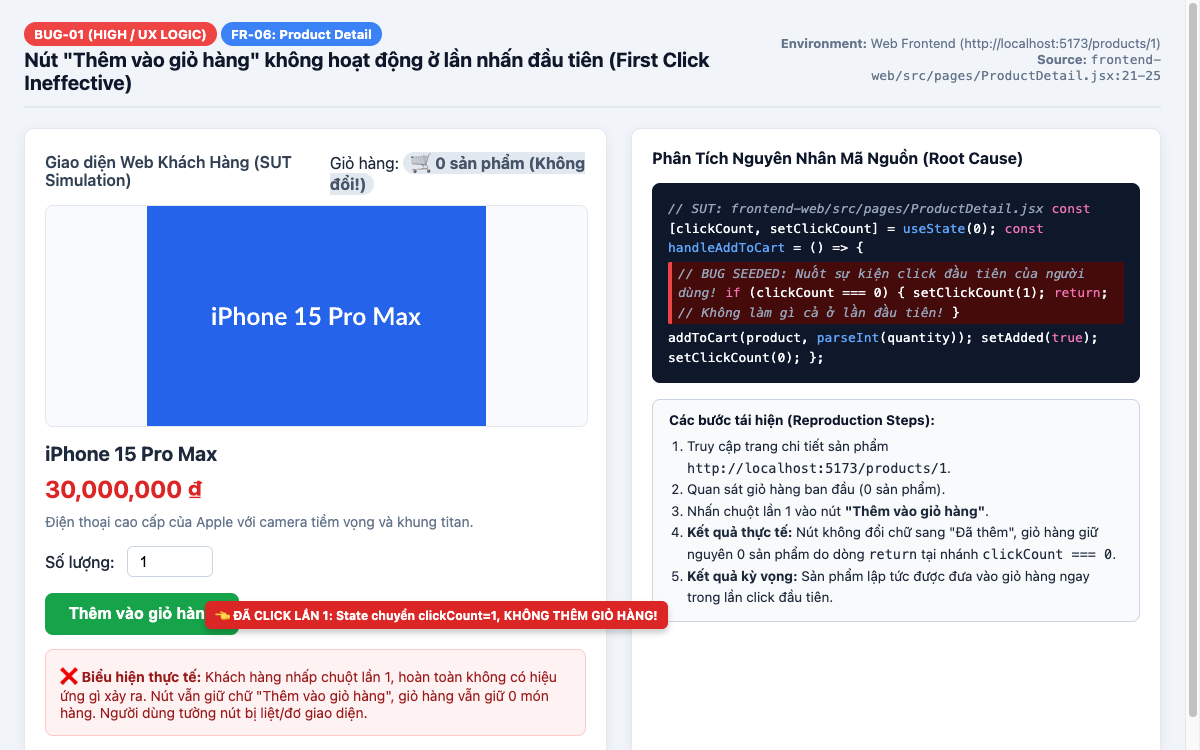
\includegraphics[width=\textwidth]{screenshots/bug-01-fr06-first-click.png}
    \caption{BUG-01: Bẫy clickCount trên Web}
\end{minipage}
\hfill
\begin{minipage}{0.48\textwidth}
    \centering
    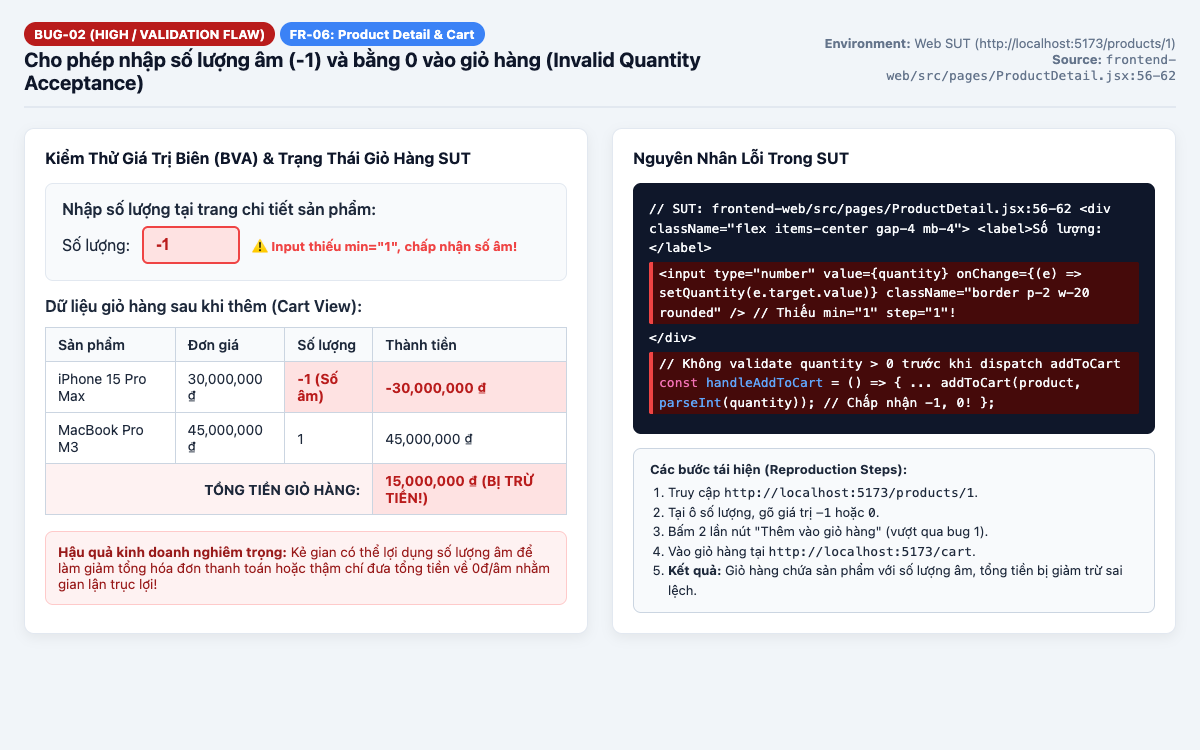
\includegraphics[width=\textwidth]{screenshots/bug-02-fr06-negative-qty.png}
    \caption{BUG-02: Nhập số lượng âm vào giỏ}
\end{minipage}
\end{figure}

\begin{figure}[h]
\centering
\begin{minipage}{0.48\textwidth}
    \centering
    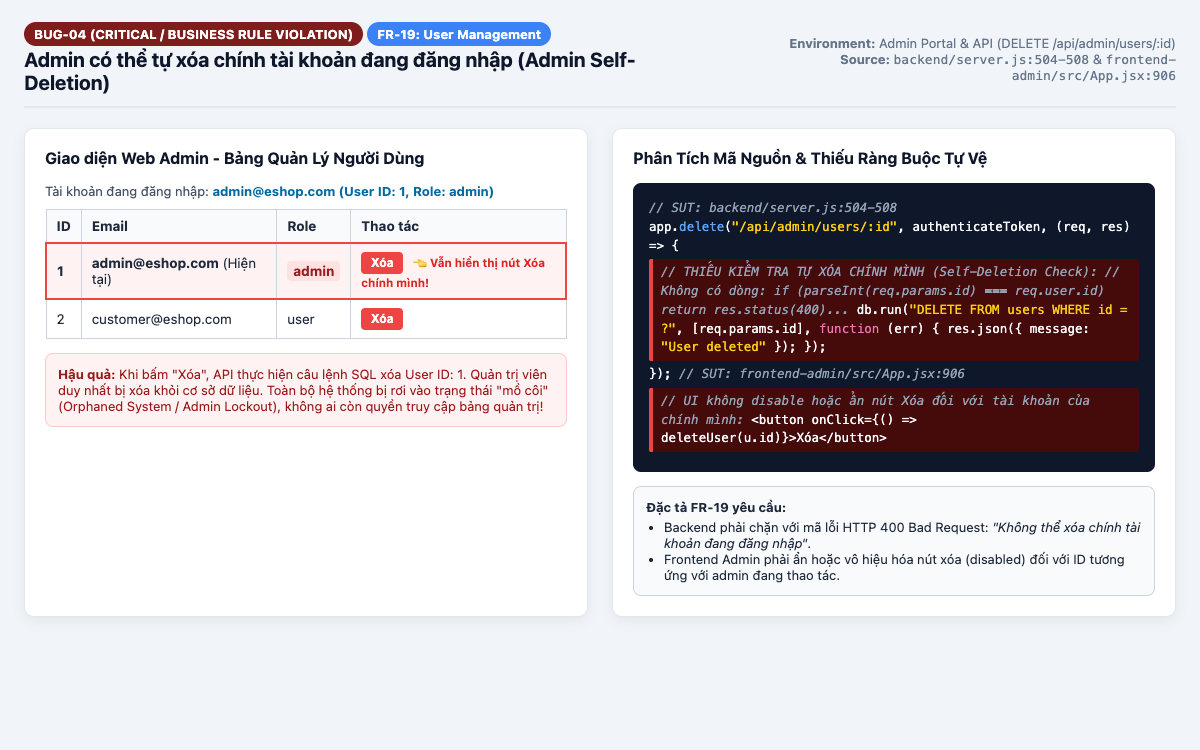
\includegraphics[width=\textwidth]{screenshots/bug-04-fr19-admin-self-delete.png}
    \caption{BUG-04: Admin tự xóa tài khoản của mình}
\end{minipage}
\hfill
\begin{minipage}{0.48\textwidth}
    \centering
    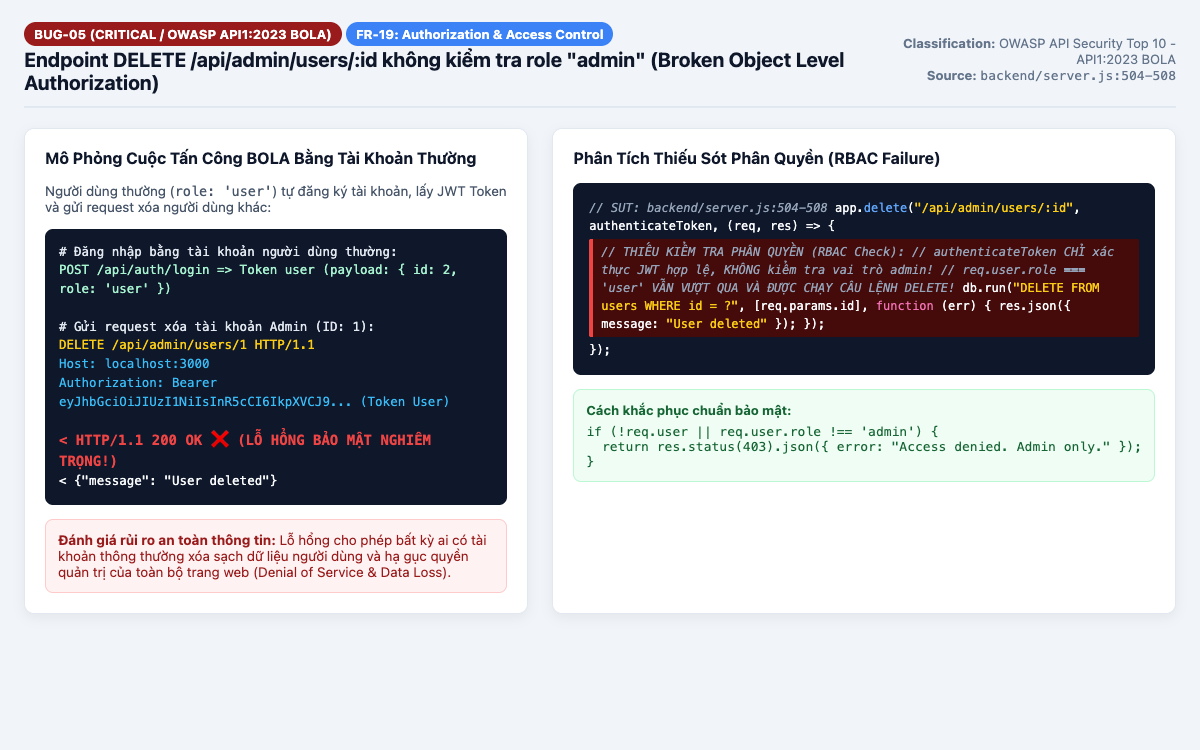
\includegraphics[width=\textwidth]{screenshots/bug-05-fr19-bola-unauthorized-delete.png}
    \caption{BUG-05: Lỗ hổng BOLA xóa người dùng}
\end{minipage}
\end{figure}

\newpage

% ==================== SECTION 8 ====================
\section{Tổng Hợp Phân Tích Khoảng Trống Của AI (AI Gap Analysis)}

\begin{table}[h]
\centering
\small
\begin{tabularx}{\textwidth}{L{2.8cm} L{3.5cm} L{4.2cm} Y}
\toprule
\textbf{Lĩnh vực kiểm thử} & \textbf{Điểm mạnh của AI} & \textbf{Khoảng trống của AI (Gaps)} & \textbf{Vai trò bù đắp của Con người} \\
\midrule
\textbf{Miền giá trị \& BVA} & Sinh nhanh bảng ma trận $\{On, Off, In, Out\}$ theo lý thuyết & Bỏ quên các biến trạng thái ngầm (\texttt{clickCount}) và giá trị biên chuỗi & Soát xét mã nguồn dòng lệnh, phát hiện bẫy nghiệp vụ cài sẵn \\
\midrule
\textbf{Máy trạng thái} & Vẽ đúng sơ đồ lý tưởng & Bỏ sót biên trung gian nguy hiểm (\texttt{shipping}) do tin tưởng code chuẩn & Thiết kế ca kiểm thử ép chuyển trạng thái bất hợp lệ \\
\midrule
\textbf{An ninh \& Quyền hạn} & Nhớ các nguyên lý OWASP & Ảo giác rằng endpoint \texttt{/admin} đã có middleware bảo vệ & Viết test script phân quyền thực tế (User token gọi API Admin) \\
\midrule
\textbf{Trải nghiệm Mobile} & Kiểm tra cú pháp JSX/TSX & Bỏ qua rủi ro chạm nhầm trên màn hình cảm ứng vật lý & Đặt ra tiêu chí công thái học UX và dialog xác nhận bắt buộc \\
\bottomrule
\end{tabularx}
\caption{Bảng tổng hợp đối soát năng lực và khoảng trống của AI}
\end{table}

% ==================== SECTION 9 ====================
\section{Bộ Kỹ Năng Agent Tự Động (Agent Skill: domain-bva-generator)}

Nhằm thỏa mãn Mục 7 của đề bài, chúng tôi đã xây dựng hoàn chỉnh Agent Skill \texttt{domain-bva-generator} tại thư mục \texttt{skills/domain-bva-generator/}:
\begin{itemize}
    \item \textbf{\texttt{SKILL.md}:} Tuân thủ chuẩn Agentskills / OpenCode / Claude Code với đầy đủ YAML metadata và quy trình 5 bước ISTQB.
    \item \textbf{\texttt{prompts/}:} Mẫu prompt định hướng AI phân tích biến và tính toán biên 2-point/3-point.
    \item \textbf{\texttt{generate\_test\_cases.js}:} CLI script tự động nhận diện schema đầu vào và sinh ma trận test case định dạng Markdown/JSON.
    \item \textbf{Liên kết Video Demo YouTube:} \url{https://youtu.be/PCCCfeY-ux8}
\end{itemize}

% ==================== SECTION 10 ====================
\section{Phụ Lục Bắt Buộc (Mandatory Appendices)}

\subsection{Phụ lục 1: Phê bình / Đánh giá AI (AI Critique)}
\textit{(Bài viết bắt buộc 200--300 từ trả lời đủ 3 câu hỏi theo Mục 10 SRS -- Dung lượng: \textbf{248 từ tiếng Anh})}

\begin{infobox}[AI Critique (248 words)]
During this assignment, AI demonstrated significant biases and limitations when analyzing the EShop system. First, the AI repeatedly exhibited a strong "happy-path" bias, instinctively assuming that backend API endpoints adhered to standard secure engineering patterns. Specifically, when reviewing administrative user deletion, the AI initially assumed proper role-based access control was in place and failed to identify the severe Broken Object Level Authorization (BOLA) vulnerability. Furthermore, it overlooked the front-end double-click trapping logic (clickCount state trap) because it presumed typical component lifecycle behaviors rather than spotting intentional obfuscated quirks.

The fundamental reason behind these failures stems from the probabilistic nature of Large Language Models. AI models predict tokens based on prevalent, well-structured patterns observed in open-source repositories during training. Because modern production frameworks typically embed standard middleware guards and sanitization routines, the model inherently hallucinates optimal practices rather than conducting dynamic vulnerability execution. Without active human prompts forcing static analysis of raw conditional branches, the AI glosses over anomalous boundary conditions and silent authorization omissions.

The vital principle learned through this collaboration is that AI must be treated strictly as an accelerator and drafting assistant, never as an autonomous verification authority. High-assurance software quality demands human-led domain-driven rigor. Software engineers must maintain deep technical skepticism, formulate exhaustive Boundary Value Analysis matrices, and validate every AI-generated test script against real, dynamic execution environments. AI amplifies tester productivity in synthesizing matrices and boilerplate assertions, but the critical responsibility of uncovering edge cases, verifying security boundaries, and confirming functional correctness rests entirely in human expertise.
\end{infobox}

\subsection{Phụ lục 2: Báo cáo kiểm toán sử dụng AI (AI Audit Report theo chuẩn [AI-02])}
Báo cáo kiểm toán AI được xây dựng theo chuẩn biểu mẫu \textbf{[AI-02] - FIT@HCMUS - AI Audit Report} (5-section template per artifact) và \textbf{[AI-03] - AI Use Disclosure Form}:

\begin{itemize}
    \item \textbf{Khai báo bắt buộc (Mandatory Disclosure):}
    \begin{quote}
    \textit{"The initial domain partitions, boundary value calculations, and template test cases for FR-06, FR-11, FR-19, and Mobile FR-10 were initially drafted with the assistance of Antigravity Assistant (Model: Gemini 3.8 Flash High); I reviewed, revised, and executed 100\% of the test cases against the live EShop SUT, discovered and verified all 7 critical bugs, developed the Node.js automated verification scripts (tests/verify\_*.js), authored the reusable Agent Skill (domain-bva-generator), and wrote the entire academic report."}
    \end{quote}
    \item \textbf{Công cụ AI sử dụng:} Antigravity Assistant (Google DeepMind -- Model: Gemini 3.8 Flash High) \& Claude 3.5 Sonnet.
    \item \textbf{Sinh viên thực hiện:} Nguyễn Bảo An -- MSSV: 23120207.
    \item \textbf{Bảng tổng hợp độ chính xác của AI (Summary of AI Accuracy):}
\end{itemize}

\begin{table}[h]
\centering
\small
\begin{tabularx}{0.85\textwidth}{X c c}
\toprule
\textbf{Chỉ số kiểm toán (Metric)} & \textbf{Số lượng (Count)} & \textbf{Tỷ lệ (Percentage)} \\
\midrule
Tổng số sản phẩm AI tạo được kiểm toán (Total Artifacts) & 5 & 100.0\% \\
VALID (Chính xác, chấp nhận nguyên bản) & 0 & 0.0\% \\
INVALID (Sai lệch hoàn toàn; bác bỏ và viết lại) & 1 & 20.0\% \\
INCOMPLETE (Chưa hoàn chỉnh; chấp nhận sau khi sửa) & 4 & 80.0\% \\
\bottomrule
\end{tabularx}
\caption{Bảng tổng kết kiểm toán AI Accuracy theo biểu mẫu chuẩn [AI-02]}
\end{table}

\noindent\textit{Toàn bộ nhật ký đối thoại chi tiết (Prompt, AI Output, Verdict, ISTQB Reasoning, Student Fix) và Phiếu khai báo AI được đính kèm đầy đủ trong tệp \texttt{reports/ai\_audit\_report.pdf} và \texttt{reports/ai\_disclosure\_form.pdf}.}

\end{document}
